\documentclass[aspectratio=169, 10pt]{beamer}

% --- GÓI HỌC THUẬT & FONT TIẾNG VIỆT CHO XELATEX ---
\usepackage{fontspec}
\setmainfont{Arial}
\setsansfont{Arial}
\setmonofont{Consolas}

\usepackage{amsmath,amssymb}
\usepackage{graphicx}
\usepackage{booktabs}
\usepackage{tabularx}
\usepackage{multicol}
\usepackage{listings}
\usepackage{xcolor}
\usepackage{tikz}
\usepackage{tcolorbox}
\tcbuselibrary{skins,breakable,listings}

% --- ĐỊNH NGHĨA MÀU SẮC CHUẨN ĐẠI HỌC ---
\definecolor{UniNavy}{RGB}{15, 44, 89}        % Xanh hải quân chủ đạo (#0F2C59)
\definecolor{UniBlue}{RGB}{29, 93, 155}       % Xanh Slate (#1D5D9B)
\definecolor{UniLightBlue}{RGB}{220, 235, 252}% Nền xanh nhạt
\definecolor{UniOrange}{RGB}{225, 112, 18}    % Cam nhấn mạnh (#E17012)
\definecolor{UniGreen}{RGB}{34, 139, 34}      % Xanh lá thực hành
\definecolor{UniDark}{RGB}{33, 37, 41}        % Màu chữ chính / nền console
\definecolor{CodeBg}{RGB}{248, 249, 250}      % Nền code
\definecolor{JavaKeyword}{RGB}{127, 0, 85}    % Màu tím từ khóa Java
\definecolor{JavaString}{RGB}{42, 0, 255}     % Màu xanh chuỗi Java
\definecolor{JavaComment}{RGB}{63, 127, 95}   % Màu xanh lá chú thích Java

% --- CẤU HÌNH THEME BEAMER HIỆN ĐẠI ---
\usetheme{Madrid}
\usecolortheme{whale}

\setbeamercolor{palette primary}{bg=UniNavy, fg=white}
\setbeamercolor{palette secondary}{bg=UniBlue, fg=white}
\setbeamercolor{palette tertiary}{bg=UniNavy!85, fg=white}
\setbeamercolor{palette quaternary}{bg=UniNavy, fg=white}

\setbeamercolor{structure}{fg=UniNavy}
\setbeamercolor{titlelike}{parent=structure, fg=UniNavy}
\setbeamercolor{frametitle}{bg=UniNavy, fg=white}
\setbeamercolor{frametitle continuation}{fg=white}
\setbeamercolor{normal text}{fg=UniDark}

% Cấu hình khối thông tin (Blocks)
\setbeamercolor{block title}{bg=UniBlue, fg=white}
\setbeamercolor{block body}{bg=UniLightBlue!40, fg=UniDark}
\setbeamercolor{block title example}{bg=UniGreen, fg=white}
\setbeamercolor{block body example}{bg=UniGreen!10, fg=UniDark}
\setbeamercolor{block title alerted}{bg=UniOrange, fg=white}
\setbeamercolor{block body alerted}{bg=UniOrange!10, fg=UniDark}

% Cấu hình Footline chuyên nghiệp
\setbeamertemplate{navigation symbols}{}
\setbeamertemplate{footline}{
  \leavevmode%
  \hbox{%
    \begin{beamercolorbox}[wd=.333333\paperwidth,ht=2.5ex,dp=1.1ex,left,leftskip=2ex]{author in head/foot}%
      \usebeamerfont{author in head/foot}\textbf{Lớp IT26M} | Lập trình Java
    \end{beamercolorbox}%
    \begin{beamercolorbox}[wd=.333333\paperwidth,ht=2.5ex,dp=1.1ex,center]{title in head/foot}%
      \usebeamerfont{title in head/foot}Chương 1: Introduction to Java
    \end{beamercolorbox}%
    \begin{beamercolorbox}[wd=.333333\paperwidth,ht=2.5ex,dp=1.1ex,right,rightskip=2ex]{date in head/foot}%
      \usebeamerfont{date in head/foot}\insertframenumber{} / \inserttotalframenumber
    \end{beamercolorbox}%
  }%
  \vskip0pt%
}

% --- CẤU HÌNH GÓI LISTINGS CHO JAVA & TERMINAL ---
\lstset{
  language=Java,
  basicstyle=\ttfamily\scriptsize,
  keywordstyle=\color{JavaKeyword}\bfseries,
  stringstyle=\color{JavaString},
  commentstyle=\color{JavaComment}\itshape,
  numbers=left,
  numberstyle=\tiny\color{gray},
  stepnumber=1,
  numbersep=6pt,
  backgroundcolor=\color{CodeBg},
  frame=single,
  rulecolor=\color{black!20},
  tabsize=4,
  showstringspaces=false,
  breaklines=true,
  breakatwhitespace=true,
  columns=flexible,
  keepspaces=true,
  xleftmargin=12pt,
  framexleftmargin=10pt
}

% Style cho console output
\lstdefinestyle{terminalStyle}{
  basicstyle=\ttfamily\scriptsize\color{white},
  backgroundcolor=\color{UniDark},
  frame=single,
  rulecolor=\color{UniDark},
  numbers=none,
  breaklines=true,
  showstringspaces=false,
  xleftmargin=6pt,
  framexleftmargin=6pt
}

% --- THÔNG TIN BÀI GIẢNG ---
\title[\textbf{Chương 1: Introduction to Java}]{\textbf{\LARGE KỸ THUẬT LẬP TRÌNH / JAVA}}
\subtitle{\textbf{\large CHƯƠNG 1: INTRODUCTION TO JAVA PROGRAMMING}\\[2mm]
\small\textcolor{UniLightBlue}{Buổi học tích hợp Lý thuyết \& Thực hành tại lớp (Thời lượng: 3 Tiết)}}
\author[\textbf{Khoa CNTT - Lớp IT26M}]{\textbf{Giảng viên Học phần} \\ \footnotesize Khoa Công nghệ Thông tin}
\institute[\textbf{UDA}]{\textbf{Dành cho sinh viên Khóa 2026 -- Lớp IT26M}\\[1mm]
\scriptsize Dựa trên giáo trình: \textit{Building Java Programs} (Stuart Reges \& Marty Stepp)}
\date{\textbf{Năm học 2026}}

\begin{document}

% ==============================================================================
% SLIDE 1: TRANG TIÊU ĐỀ
% ==============================================================================
\begin{frame}[plain]
  \titlepage
\end{frame}

% ==============================================================================
% SLIDE 2: MỤC TIÊU BÀI HỌC (CLOs)
% ==============================================================================
\begin{frame}{Mục tiêu học tập bài học (Course Learning Outcomes -- CLOs)}
  \begin{block}{\textbf{Chuẩn đầu ra sau khi hoàn thành Chương 1 (Buổi học 3 tiết):}}
    \begin{itemize}
      \item[\checkmark] \textbf{CLO 1.1 (Hiểu):} Giải thích bản chất kiến trúc máy tính, hệ nhị phân, cơ chế biên dịch vs. thông dịch, vai trò của \textbf{máy ảo JVM} và mã \textbf{Bytecode} (WORA).
      \item[\checkmark] \textbf{CLO 1.2 (Áp dụng):} Viết thành thạo khung chương trình Java cơ bản (\texttt{class}, \texttt{main}), phân biệt \texttt{print} và \texttt{println}, sử dụng chính xác các \textbf{ký tự thoát} (\texttt{\textbackslash n, \textbackslash t, \textbackslash", \textbackslash\textbackslash}).
      \item[\checkmark] \textbf{CLO 1.3 (Phân tích):} Nhận diện và phân loại chính xác \textbf{3 loại lỗi} (Syntax, Runtime, Logic); đọc thông báo lỗi từ trình biên dịch để gỡ lỗi (debug).
      \item[\checkmark] \textbf{CLO 1.4 (Thiết kế):} Vận dụng tư duy \textbf{Phân rã thủ tục (Procedural Decomposition)} và nguyên lý \textbf{DRY}; khai báo và gọi phương thức tĩnh (\texttt{static methods}); phân tích luồng điều khiển (\textit{Flow of Control}).
      \item[\checkmark] \textbf{CLO 1.5 (Sáng tạo):} Độc lập viết, biên dịch qua CLI (\texttt{javac}/\texttt{java}) và IDE một chương trình hoàn chỉnh vẽ hình nghệ thuật ASCII có cấu trúc nhiều cấp.
    \end{itemize}
  \end{block}
\end{frame}

% ==============================================================================
% SLIDE 3: NỘI DUNG & TIẾN TRÌNH BUỔI HỌC (3 TIẾT)
% ==============================================================================
\begin{frame}{Lộ trình buổi học 3 tiết (Tích hợp Lý thuyết \& Thực hành)}
  \begin{columns}[t]
    \column{0.32\textwidth}
    \begin{tcolorbox}[colback=UniNavy!10,colframe=UniNavy,title=\textbf{TIẾT 1 (50 phút)},fonttitle=\small\bfseries]
      \footnotesize
      \textbf{Nền tảng \& Khởi đầu:}
      \begin{itemize}
        \item Khái niệm tính toán \& Nhị phân
        \item Compiler vs. Interpreter
        \item Kiến trúc JVM \& Bytecode
        \item Quy trình: Edit-Compile-Run
        \item Chương trình \texttt{Hello.java}
        \item Lệnh \texttt{print} vs \texttt{println}
      \end{itemize}
      \vspace{1mm}
      \textbf{\textcolor{UniNavy}{[Lab 1]:}} Viết \& chạy Java trên CLI và IDE.
    \end{tcolorbox}

    \column{0.32\textwidth}
    \begin{tcolorbox}[colback=UniBlue!10,colframe=UniBlue,title=\textbf{TIẾT 2 (50 phút)},fonttitle=\small\bfseries]
      \footnotesize
      \textbf{Cú pháp \& Gỡ lỗi:}
      \begin{itemize}
        \item Ký tự thoát (\textit{Escape Seq})
        \item Định danh, Từ khóa, CamelCase
        \item Quy ước chú thích (Comments)
        \item Phân loại 3 nhóm lỗi:
          \begin{itemize}\scriptsize
            \item Lỗi cú pháp (Syntax)
            \item Lỗi thực thi (Runtime)
            \item Lỗi ngữ nghĩa (Logic)
          \end{itemize}
        \item Chiến lược đọc lỗi \& gỡ lỗi
      \end{itemize}
      \vspace{1mm}
      \textbf{\textcolor{UniBlue}{[Lab 2]:}} Thử thách Debug \& Escape Strings.
    \end{tcolorbox}

    \column{0.32\textwidth}
    \begin{tcolorbox}[colback=UniGreen!10,colframe=UniGreen,title=\textbf{TIẾT 3 (50 phút)},fonttitle=\small\bfseries]
      \footnotesize
      \textbf{Phân rã \& Case Study:}
      \begin{itemize}
        \item Tư duy phân rã Top-down
        \item Phương thức tĩnh (\texttt{static})
        \item Luồng điều khiển (\textit{Control Flow})
        \item Mục tiêu: Structure \& DRY
        \item Case Study \texttt{DrawFigures}:
          \begin{itemize}\scriptsize
            \item Bản 1: Naïve (đơn khối)
            \item Bản 2: Phân rã cấp 1
            \item Bản 3: Phân rã triệt để
          \end{itemize}
      \end{itemize}
      \vspace{1mm}
      \textbf{\textcolor{UniGreen}{[Lab 3]:}} Mini Project vẽ Tàu Rocket.
    \end{tcolorbox}
  \end{columns}
\end{frame}

% ==============================================================================
% PHẦN I: TIẾT 1
% ==============================================================================
\section{Tiết 1: Nền tảng Tính toán \& Chương trình Java Đầu tiên}

\begin{frame}[plain]
  \begin{center}
    \vspace{1.5cm}
    {\Huge \textcolor{UniNavy}{\textbf{TIẾT 1}}}\\[4mm]
    {\Large \textbf{NỀN TẢNG HỆ THỐNG TÍNH TOÁN, KIẾN TRÚC MÁY ẢO JVM}}\\[2mm]
    {\large \textbf{\& XÂY DỰNG CHƯƠNG TRÌNH JAVA ĐẦU TIÊN}}\\[6mm]
    \rule{0.5\textwidth}{1pt}\\[4mm]
    \textit{\small Thời lượng: 50 phút | 35' Lý thuyết tương tác + 15' Hands-on Lab 1}
  \end{center}
\end{frame}

% ------------------------------------------------------------------------------
\begin{frame}{1.1 Tại sao chúng ta cần học lập trình? (Why Programming?)}
  \begin{columns}
    \column{0.55\textwidth}
    \begin{block}{\textbf{Bản chất của khoa học máy tính}}
      \begin{quote}
        ``Người ta thường nói rằng một người không thực sự hiểu điều gì đó cho đến khi họ dạy nó cho người khác. Trên thực tế, một người \textbf{không thực sự hiểu} điều gì đó cho đến khi họ \textbf{dạy nó cho một chiếc máy tính}, tức là diễn đạt nó dưới dạng một thuật toán.''
        \flushright{\footnotesize --- Donald Knuth (Turing Award, Cha đẻ ngành Phân tích thuật toán)}
      \end{quote}
    \end{block}
    \vspace{2mm}
    \begin{itemize}
      \item \textbf{Máy tính:} Thiết bị phần cứng vạn năng (General-purpose device).
      \item \textbf{Chương trình (Program):} Tập hợp các chỉ thị ra lệnh cho phần cứng.
      \item \textbf{Lập trình:} Rèn luyện tư duy giải quyết vấn đề có cấu trúc.
    \end{itemize}

    \column{0.45\textwidth}
    \begin{tcolorbox}[colback=white,colframe=UniBlue,title=\textbf{Thành phần cốt lõi của máy tính}]
      \small
      \begin{itemize}
        \item \textbf{CPU (Bộ vi xử lý trung tâm):} ``Bộ não'' thực thi các phép tính logic và số học.
        \item \textbf{Bộ nhớ chính (RAM):} Lưu trữ tạm thời, tốc độ cực nhanh, mất dữ liệu khi mất nguồn.
        \item \textbf{Bộ nhớ thứ cấp (Ổ cứng/SSD):} Lưu trữ dữ liệu vĩnh viễn (persistent storage).
        \item \textbf{Thiết bị I/O:} Bàn phím, chuột, màn hình, kết nối mạng.
      \end{itemize}
    \end{tcolorbox}
  \end{columns}
\end{frame}

% ------------------------------------------------------------------------------
\begin{frame}{Thế giới số \& Biểu diễn dữ liệu bằng Hệ nhị phân (Binary)}
  \begin{columns}
    \column{0.5\textwidth}
    \begin{block}{\textbf{Tại sao máy tính sử dụng số nhị phân?}}
      \begin{itemize}
        \item Phần cứng vật lý cấu tạo từ hàng tỷ bóng bán dẫn (\textit{transistors}).
        \item Hai trạng thái vật lý ổn định nhất:
          \begin{itemize}
            \item \textbf{Bật (On) / Điện áp cao:} Đại diện cho số \textbf{1}.
            \item \textbf{Tắt (Off) / Điện áp thấp:} Đại diện cho số \textbf{0}.
          \end{itemize}
        \item \textbf{Bit (Binary Digit):} Đơn vị thông tin nhỏ nhất (0 hoặc 1).
        \item \textbf{Byte:} Nhóm 8 bits. 1 Byte biểu diễn được $2^8 = 256$ trạng thái (từ 0 đến 255).
      \end{itemize}
    \end{block}

    \column{0.5\textwidth}
    \begin{exampleblock}{\textbf{Cơ chế biểu diễn số theo cơ số 2}}
      So sánh hệ thập phân (Base-10) và nhị phân (Base-2):
      \vspace{2mm}
      \centering
      \begin{tabular}{ccccc}
        \toprule
        \textbf{Trọng số} & $2^3 = 8$ & $2^2 = 4$ & $2^1 = 2$ & $2^0 = 1$ \\
        \midrule
        \textbf{Bit} & \textbf{1} & \textbf{0} & \textbf{1} & \textbf{1} \\
        \bottomrule
      \end{tabular}
      \vspace{2mm}
      \begin{align*}
        (1011)_2 &= 1 \times 8 + 0 \times 4 + 1 \times 2 + 1 \times 1 \\
                 &= 8 + 0 + 2 + 1 = \mathbf{11}_{10}
      \end{align*}
      \footnotesize
      $\to$ Mọi chương trình, hình ảnh, video, âm thanh cuối cùng đều được ánh xạ về các dãy bit 0 và 1!
    \end{exampleblock}
  \end{columns}
\end{frame}

% ------------------------------------------------------------------------------
\begin{frame}{Cơ chế thực thi: Trình biên dịch (Compiler) vs. Thông dịch (Interpreter)}
  \begin{columns}[t]
    \column{0.5\textwidth}
    \begin{block}{\textbf{Trình biên dịch truyền thống (C/C++)}}
      \begin{itemize}
        \item Dịch toàn bộ mã nguồn (\textit{Source code}) thành \textbf{Mã máy trực tiếp (Native Machine Code)}.
        \item \textbf{Ưu điểm:} Tốc độ thực thi cực nhanh, tối ưu phần cứng.
        \item \textbf{Nhược điểm chí tử:} \textcolor{red}{\textbf{Phụ thuộc nền tảng!}} File thực thi trên Intel x86 Windows không thể chạy trên ARM macOS hay Linux.
      \end{itemize}
    \end{block}

    \column{0.5\textwidth}
    \begin{block}{\textbf{Trình thông dịch (Python, JavaScript)}}
      \begin{itemize}
        \item Đọc và diễn giải trực tiếp từng dòng lệnh tại thời điểm chạy.
        \item \textbf{Ưu điểm:} Linh hoạt, dễ thử nghiệm trực tiếp.
        \item \textbf{Nhược điểm:} Tốc độ thực thi chậm hơn nhiều so với mã đã biên dịch sẵn.
      \end{itemize}
    \end{block}
  \end{columns}

  \vspace{3mm}
  \begin{alertblock}{\textbf{Câu hỏi đặt ra cho các nhà thiết kế ngôn ngữ Java (Năm 1995)}}
    Làm sao vừa đạt được tốc độ thực thi cao, vừa có thể chạy trên \textbf{mọi nền tảng phần cứng} mà không cần biên dịch lại?
  \end{alertblock}
\end{frame}

% ------------------------------------------------------------------------------
\begin{frame}{Kiến trúc đột phá của Java: Máy ảo JVM \& Mã Bytecode}
  \begin{columns}
    \column{0.52\textwidth}
    \begin{block}{\textbf{Triết lý: ``Write Once, Run Anywhere'' (WORA)}}
      \begin{itemize}
        \item Java kết hợp cả \textbf{Biên dịch} lẫn \textbf{Máy ảo}!
        \item Trình biên dịch Java (\texttt{javac}) không dịch ra mã máy thật của CPU.
        \item Nó dịch mã nguồn (\texttt{.java}) thành \textbf{Java Bytecode} (\texttt{.class}).
        \item Bytecode là tập lệnh chuẩn cho một cỗ máy lý thuyết gọi là \textbf{Java Virtual Machine (JVM)}.
        \item Mỗi hệ điều hành (Windows, Linux, macOS) có một bản JVM riêng biệt để thông dịch/JIT-compile Bytecode ra mã máy phần cứng.
      \end{itemize}
    \end{block}

    \column{0.48\textwidth}
    \begin{tcolorbox}[colback=white,colframe=UniBlue,title=\textbf{Bộ công cụ Java (Phân biệt JDK, JRE, JVM)}]
      \small
      \begin{itemize}
        \item \textbf{JVM (Java Virtual Machine):} Môi trường thực thi Bytecode.
        \item \textbf{JRE (Java Runtime Environment):} Gồm JVM + Thư viện chuẩn (\textit{Java Class Libraries}) để người dùng chạy ứng dụng.
        \item \textbf{JDK (Java Development Kit):} Dành cho lập trình viên! Chứa JRE + Trình biên dịch (\texttt{javac}) + Công cụ gỡ lỗi.
      \end{itemize}
      \centering
      \vspace{1mm}
      \fbox{\textbf{JDK = JRE + Tools}} $\supset$ \fbox{\textbf{JRE = JVM + Libs}}
    \end{tcolorbox}
  \end{columns}
\end{frame}

% ------------------------------------------------------------------------------
\begin{frame}{Quy trình phát triển chương trình Java: Edit $\to$ Compile $\to$ Run}
  \begin{columns}
    \column{0.55\textwidth}
    \begin{center}
      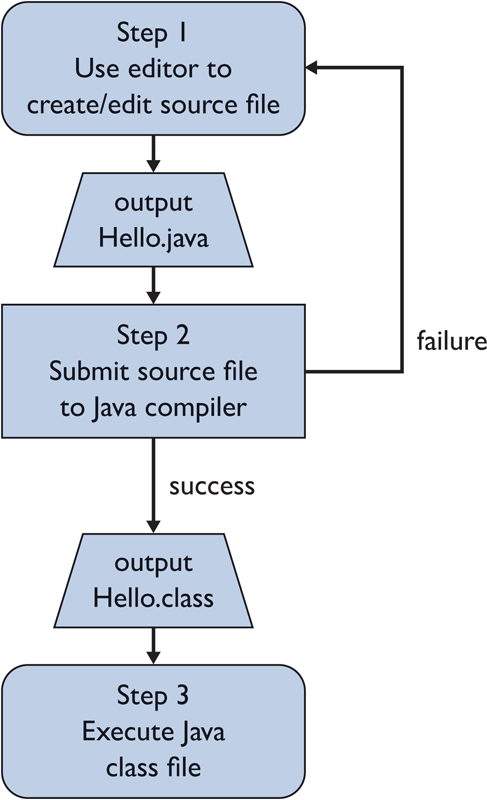
\includegraphics[width=0.82\textwidth,height=0.78\textheight,keepaspectratio]{images/fig1_1_java_execution.png}\\[1mm]
      \tiny\textit{Hình 1.1: Quá trình tạo và thực thi chương trình Java (Trích giáo trình Chapter 1, p.21)}
    \end{center}

    \column{0.45\textwidth}
    \begin{block}{\textbf{3 Bước cốt lõi của mọi lập trình viên Java:}}
      \begin{enumerate}
        \item \textbf{Bước 1: Soạn thảo (Edit)}
          \begin{itemize}\footnotesize
            \item Viết mã nguồn vào file văn bản thuần.
            \item Bắt buộc đuôi file: \texttt{Hello.java}.
          \end{itemize}
        \item \textbf{Bước 2: Biên dịch (Compile)}
          \begin{itemize}\footnotesize
            \item Lệnh: \texttt{javac Hello.java}
            \item Kiểm tra lỗi cú pháp.
            \item Tạo ra file bytecode: \texttt{Hello.class}.
          \end{itemize}
        \item \textbf{Bước 3: Thực thi (Run)}
          \begin{itemize}\footnotesize
            \item Khởi động máy ảo JVM: \texttt{java Hello}
            \item JVM nạp bytecode và chuyển cho CPU thực thi.
            \item Kết quả xuất hiện trên màn hình!
          \end{itemize}
      \end{enumerate}
    \end{block}
  \end{columns}
\end{frame}

% ------------------------------------------------------------------------------
\begin{frame}[fragile]{1.2 Chương trình Java hoàn chỉnh đầu tiên}
  \begin{columns}
    \column{0.52\textwidth}
    \begin{lstlisting}[caption={File: Hello.java}]
// Chuong trinh Java dau tien cua lop IT26M
public class Hello {
    public static void main(String[] args) {
        System.out.println("Hello, world!");
    }
}
    \end{lstlisting}
    \vspace{-2mm}
    \begin{block}{\textbf{Quy tắc vàng bắt buộc:}}
      \begin{itemize}\footnotesize
        \item Mọi mã nguồn Java đều phải nằm \textbf{bên trong một lớp (class)}.
        \item Tên file \textbf{bắt buộc phải trùng khớp 100\%} với tên lớp công khai:
          \begin{center}
            Lớp \texttt{public class \textbf{Hello}} $\Longleftrightarrow$ File \texttt{\textbf{Hello}.java}
          \end{center}
        \item Java phân biệt chữ hoa và chữ thường (\textit{case-sensitive}).
      \end{itemize}
    \end{block}

    \column{0.48\textwidth}
    \begin{tcolorbox}[colback=white,colframe=UniNavy,title=\textbf{Cấu trúc mẫu (Syntax Template)}]
      \small
      \textbf{Khai báo lớp chuẩn:}\\
      \texttt{public class \textcolor{JavaKeyword}{<TênLớp>} \{}\\
      \quad \textcolor{gray}{\textit{... các phương thức ...}}\\
      \texttt{\}}\\[3mm]
      \textbf{Cặp ngoặc nhọn \texttt{\{ \}} :}\\
      Đóng gói phạm vi (\textit{scope}) của khối lệnh. Mọi ngoặc mở \texttt{\{} đều phải có ngoặc đóng \texttt{\}} tương ứng.
    \end{tcolorbox}
  \end{columns}
\end{frame}

% ------------------------------------------------------------------------------
\begin{frame}{Mổ xẻ phương thức \texttt{main} -- Điểm bắt đầu của mọi ứng dụng}
  \begin{block}{\textbf{Dòng lệnh then chốt:}}
    \centering
    \large\texttt{\textbf{\textcolor{JavaKeyword}{public static void} main(\textcolor{UniBlue}{String}[] args) \{ ... \}}}
  \end{block}

  \vspace{2mm}
  \begin{tabularx}{\textwidth}{l p{3.2cm} X}
    \toprule
    \textbf{Từ khóa} & \textbf{Ý nghĩa học thuật} & \textbf{Diễn giải dành cho sinh viên mới học} \\
    \midrule
    \texttt{\textbf{public}} & Quyền truy cập công khai & Bất kỳ đối tượng nào (bao gồm máy ảo JVM) cũng có thể gọi phương thức này từ bên ngoài. \\
    \texttt{\textbf{static}} & Phương thức tĩnh cấp lớp & Có thể thực thi trực tiếp từ lớp mà không cần khởi tạo đối tượng (\textit{instance}). \\
    \texttt{\textbf{void}} & Kiểu dữ liệu trả về & Phương thức này thực hiện công việc và \textbf{không trả lại} giá trị nào. \\
    \texttt{\textbf{main}} & Tên phương thức & Tên quy ước đặc biệt mà JVM tìm kiếm đầu tiên khi chạy chương trình. \\
    \texttt{\textbf{String[] args}} & Mảng tham số dòng lệnh & Cho phép truyền các chuỗi đối số từ bên ngoài khi khởi động chương trình. \\
    \bottomrule
  \end{tabularx}
\end{frame}

% ------------------------------------------------------------------------------
\begin{frame}[fragile]{Lệnh xuất dữ liệu: \texttt{println} vs. \texttt{print}}
  \begin{columns}[t]
    \column{0.48\textwidth}
    \begin{block}{\textbf{System.out.println(...)}}
      In nội dung ra console và \textbf{tự động xuống dòng mới} (newline).
      \begin{lstlisting}
System.out.println("Dong thu nhat");
System.out.println("Dong thu hai");
      \end{lstlisting}
      \textbf{Kết quả trên màn hình:}
      \begin{lstlisting}[style=terminalStyle]
Dong thu nhat
Dong thu hai
      \end{lstlisting}
    \end{block}

    \column{0.48\textwidth}
    \begin{block}{\textbf{System.out.print(...)}}
      In nội dung ra console và \textbf{giữ nguyên con trỏ} ở cuối dòng hiện tại.
      \begin{lstlisting}
System.out.print("Xin ");
System.out.print("chao ");
System.out.println("IT26M!");
      \end{lstlisting}
      \textbf{Kết quả trên màn hình:}
      \begin{lstlisting}[style=terminalStyle]
Xin chao IT26M!
      \end{lstlisting}
    \end{block}
  \end{columns}

  \vspace{2mm}
  \begin{alertblock}{\textbf{Lưu ý quan trọng:}}
    Lệnh \texttt{System.out.println();} (không tham số) dùng để tạo ra một dòng trống trên console. Mọi câu lệnh trong Java \textbf{bắt buộc kết thúc bằng dấu chấm phẩy \texttt{;}}!
  \end{alertblock}
\end{frame}

% ------------------------------------------------------------------------------
\begin{frame}{[CHECKPOINT 1] Kiểm tra nhanh lý thuyết Tiết 1}
  \begin{columns}
    \column{0.6\textwidth}
    \begin{exampleblock}{\textbf{Câu hỏi 1: Lệnh nào hợp lệ trong Java?}}
      \begin{enumerate}[A.]
        \item \texttt{system.out.println("Hello");}
        \item \texttt{System.Out.println("Hello");}
        \item \texttt{System.out.println("Hello");}
        \item \texttt{System.out.println(Hello);}
      \end{enumerate}
    \end{exampleblock}

    \begin{alertblock}{\textbf{Câu hỏi 2: Vai trò của file có đuôi \texttt{.class}?}}
      \begin{enumerate}[A.]
        \item Chứa mã nguồn viết bằng tiếng Anh cho lập trình viên đọc.
        \item Chứa mã Bytecode đã được biên dịch để máy ảo JVM thực thi.
        \item Là file mã máy nhị phân chạy trực tiếp trên chip Intel.
        \item Là file cấu hình môi trường của IDE.
      \end{enumerate}
    \end{alertblock}

    \column{0.4\textwidth}
    \begin{tcolorbox}[colback=white,colframe=UniGreen,title=\textbf{Giải thích đáp án}]
      \small
      \textbf{Đáp án Câu 1: C}\\
      \textit{Java phân biệt hoa thường:} \texttt{System} viết hoa chữ S, \texttt{out} và \texttt{println} viết thường. Chuỗi chữ phải nằm trong cặp nháy kép \texttt{" "}.\\[2mm]
      \textbf{Đáp án Câu 2: B}\\
      Trình biên dịch \texttt{javac} sinh ra file \texttt{.class} chứa Bytecode độc lập nền tảng cho JVM.
    \end{tcolorbox}
  \end{columns}
\end{frame}

% ------------------------------------------------------------------------------
\begin{frame}[fragile]{[HANDS-ON LAB 1] Thực hành tại chỗ: Viết, biên dịch \& chạy Java}
  \begin{tcolorbox}[colback=white,colframe=UniGreen,title=\textbf{Nhiệm vụ thực hành Tiết 1 (Thời gian: 15 phút -- Tất cả sinh viên thực hiện)}]
    \small
    \textbf{Yêu cầu 1: Thao tác Command Line (Terminal / CMD / PowerShell)}
    \begin{enumerate}\footnotesize
      \item Mở Terminal, gõ \texttt{javac -version} và \texttt{java -version} để kiểm tra JDK.
      \item Dùng trình soạn thảo (Notepad / VS Code) tạo thư mục \texttt{Lab1} và file \texttt{WelcomeIT26M.java}.
      \item Biên dịch bằng lệnh CLI: \texttt{javac WelcomeIT26M.java} $\to$ Dùng \texttt{dir} hoặc \texttt{ls} quan sát file \texttt{WelcomeIT26M.class} vừa xuất hiện!
      \item Chạy chương trình: \texttt{java WelcomeIT26M}
    \end{enumerate}
  \end{tcolorbox}

  \begin{columns}
    \column{0.55\textwidth}
    \begin{lstlisting}[caption={Mã nguồn WelcomeIT26M.java}]
public class WelcomeIT26M {
    public static void main(String[] args) {
        System.out.println("Chao mung lop IT26M den voi Java!");
        System.out.println("Viet mot lan, chay moi noi (WORA).");
    }
}
    \end{lstlisting}

    \column{0.45\textwidth}
    \textbf{Output hiển thị chính xác:}
    \begin{lstlisting}[style=terminalStyle]
Chao mung lop IT26M den voi Java!
Viet mot lan, chay moi noi (WORA).
    \end{lstlisting}
  \end{columns}
\end{frame}

% ==============================================================================
% PHẦN II: TIẾT 2
% ==============================================================================
\section{Tiết 2: Cú pháp Nâng cao, Ký tự Thoát \& Xử lý Lỗi}

\begin{frame}[plain]
  \begin{center}
    \vspace{1.5cm}
    {\Huge \textcolor{UniNavy}{\textbf{TIẾT 2}}}\\[4mm]
    {\Large \textbf{CHUỖI KÝ TỰ, KÝ TỰ THOÁT (ESCAPE SEQUENCES)}}\\[2mm]
    {\large \textbf{\& KỸ NĂNG CHẨN ĐOÁN, GỠ LỖI LẬP TRÌNH (DEBUGGING)}}\\[6mm]
    \rule{0.5\textwidth}{1pt}\\[4mm]
    \textit{\small Thời lượng: 50 phút | 35' Lý thuyết \& Thảo luận + 15' Hands-on Lab 2}
  \end{center}
\end{frame}

% ------------------------------------------------------------------------------
\begin{frame}{Chuỗi ký tự (String Literals) \& Thách thức khi xuất ký tự đặc biệt}
  \begin{columns}
    \column{0.5\textwidth}
    \begin{block}{\textbf{Chuỗi ký tự (String Literal)}}
      \begin{itemize}
        \item Là một chuỗi các ký tự nằm trong cặp \textbf{dấu ngoặc kép} (\texttt{"..."}).
        \item Ví dụ: \texttt{"Xin chao"}, \texttt{"IT26M"}, \texttt{""} (chuỗi rỗng).
        \item \textcolor{red}{\textbf{Cấm:}} Không được ngắt một chuỗi qua nhiều dòng mà không đóng ngoặc kép!
      \end{itemize}
    \end{block}

    \column{0.5\textwidth}
    \begin{alertblock}{\textbf{Vấn đề hóc búa nảy sinh:}}
      Nếu muốn in ra màn hình chính xác câu sau:
      \begin{center}
        \texttt{Giao vien noi: "Java rat thu vi!"}
      \end{center}
      Nếu viết:\\
      \texttt{System.out.println("Giao vien noi: \textcolor{red}{"Java rat thu vi!"}");}\\
      $\to$ \textbf{Trình biên dịch sẽ báo lỗi ngay!} Vì nó nghĩ chuỗi kết thúc ở dấu ngoặc kép thứ hai.
    \end{alertblock}
  \end{columns}

  \vspace{3mm}
  \begin{center}
    \textbf{Giải pháp trong mọi ngôn ngữ lập trình:} Sử dụng \textbf{Ký tự thoát (Escape Sequences)}!
  \end{center}
\end{frame}

% ------------------------------------------------------------------------------
\begin{frame}[fragile]{Bảng ký tự thoát chuẩn trong Java (Escape Sequences)}
  \begin{block}{\textbf{Quy tắc: Dấu gạch chéo ngược (\textbackslash) kết hợp với ký tự đi liền sau:}}
    \centering
    \small
    \begin{tabularx}{0.9\textwidth}{c l X}
      \toprule
      \textbf{Ký tự thoát} & \textbf{Tên gọi} & \textbf{Ý nghĩa \& Hành vi thực hiện} \\
      \midrule
      \texttt{\textbf{\textbackslash t}} & Tab & Thêm khoảng thụt lề tab (căn chỉnh cột dữ liệu đẹp mắt). \\
      \texttt{\textbf{\textbackslash n}} & Newline & Xuống dòng mới ngay tại vị trí xuất hiện. \\
      \texttt{\textbf{\textbackslash"}} & Double quote & In dấu ngoặc kép \texttt{"} mà không làm đóng chuỗi. \\
      \texttt{\textbf{\textbackslash\textbackslash}} & Backslash & In một dấu gạch chéo ngược \texttt{\textbackslash}. \\
      \bottomrule
    \end{tabularx}
  \end{block}

  \vspace{1mm}
  \begin{columns}
    \column{0.5\textwidth}
    \begin{lstlisting}[caption={Ví dụ sử dụng Escape Sequences}]
System.out.println("Cot 1\tCot 2\tCot 3");
System.out.println("Dong 1\nDong 2\nDong 3");
System.out.println("Dau \"nhay kep\" va gach \\");
    \end{lstlisting}

    \column{0.5\textwidth}
    \textbf{Kết quả in ra màn hình:}
    \begin{lstlisting}[style=terminalStyle]
Cot 1   Cot 2   Cot 3
Dong 1
Dong 2
Dong 3
Dau "nhay kep" va gach \
    \end{lstlisting}
  \end{columns}
\end{frame}

% ------------------------------------------------------------------------------
\begin{frame}{Định danh (Identifiers) \& Từ khóa chuẩn Java}
  \begin{columns}[t]
    \column{0.5\textwidth}
    \begin{block}{\textbf{Định danh (Identifiers)}}
      Tên do lập trình viên đặt cho lớp, phương thức, biến...
      \begin{itemize}\small
        \item \textbf{Ký tự hợp lệ:} Các chữ cái (\texttt{a-z, A-Z}), chữ số (\texttt{0-9}), dấu gạch dưới (\texttt{\_}), dấu đô la (\texttt{\$}).
        \item \textbf{Quy tắc 1:} \textcolor{red}{\textbf{Không được bắt đầu bằng chữ số!}} (Hợp lệ: \texttt{diem1}, không hợp lệ: \texttt{1diem}).
        \item \textbf{Quy tắc 2:} Không chứa dấu cách hoặc ký tự đặc biệt (\texttt{@, \#, \%, -, +}).
        \item \textbf{Quy tắc 3:} \textcolor{red}{\textbf{Không trùng với Từ khóa Java!}}
      \end{itemize}
    \end{block}

    \column{0.5\textwidth}
    \begin{alertblock}{\textbf{Từ khóa Java (Keywords -- Dành riêng)}}
      Java có 50+ từ khóa đặc biệt đã được định nghĩa sẵn cú pháp:
      \vspace{2mm}
      \centering
      \footnotesize
      \begin{tabular}{llll}
        \texttt{public} & \texttt{class} & \texttt{static} & \texttt{void} \\
        \texttt{int}    & \texttt{double}& \texttt{boolean}& \texttt{char} \\
        \texttt{if}     & \texttt{else}  & \texttt{for}    & \texttt{while} \\
        \texttt{return} & \texttt{new}   & \texttt{true}   & \texttt{false} \\
      \end{tabular}
      \flushleft\vspace{2mm}
      \textit{Tuyệt đối không dùng các từ trên làm tên Class hay tên hàm!}
    \end{alertblock}
  \end{columns}
\end{frame}

% ------------------------------------------------------------------------------
\begin{frame}{Phong cách lập trình chuẩn đại học: Quy ước CamelCase \& Comments}
  \begin{columns}[t]
    \column{0.5\textwidth}
    \begin{block}{\textbf{Quy ước đặt tên CamelCase}}
      \begin{itemize}\small
        \item \textbf{Tên Lớp (UpperCamelCase):}\\
          Viết hoa chữ cái đầu của mỗi từ.\\
          \textit{Ví dụ:} \texttt{Hello}, \texttt{DrawFigures3}, \texttt{StudentManager}.
        \item \textbf{Tên Phương thức \& Biến (lowerCamelCase):}\\
          Chữ cái đầu viết thường, viết hoa các từ tiếp theo.\\
          \textit{Ví dụ:} \texttt{main}, \texttt{drawDiamond}, \texttt{calculateTotalScore}.
      \end{itemize}
    \end{block}

    \column{0.5\textwidth}
    \begin{block}{\textbf{3 Loại chú thích (Comments) trong Java}}
      \begin{itemize}\small
        \item \textbf{Chú thích 1 dòng:} Bắt đầu bằng \texttt{//}\\
          \texttt{// Tinh tong diem cua sinh vien}
        \item \textbf{Chú thích nhiều dòng:} Cặp \texttt{/* ... */}\\
          \texttt{/* Tac gia: IT26M} \\
          \texttt{\phantom{/* }Ngay tao: 2026 */}
        \item \textbf{Chú thích tài liệu (Javadoc):} Cặp \texttt{/** ... */}\\
          Dùng để sinh tài liệu API tự động.
      \end{itemize}
    \end{block}
  \end{columns}

  \vspace{2mm}
  \begin{center}
    \small\textit{``Mã nguồn viết ra cho người đọc hiểu trước, máy tính hiểu sau.'' -- Thụt lề (\textbf{Indentation}) nhất quán 4 khoảng trắng!}
  \end{center}
\end{frame}

% ------------------------------------------------------------------------------
\begin{frame}{1.3 Phân loại lỗi lập trình: 3 nhóm lỗi kinh điển}
  \begin{center}
    Mọi lập trình viên từ sinh viên năm nhất đến chuyên gia thâm niên đều phải đối mặt với lỗi!
  \end{center}
  \vspace{1mm}
  \begin{columns}[t]
    \column{0.32\textwidth}
    \begin{tcolorbox}[colback=red!10,colframe=red!80!black,title=\textbf{1. Lỗi Cú pháp\\(Syntax Errors)},fonttitle=\small\bfseries]
      \footnotesize
      \begin{itemize}
        \item Xảy ra trong giai đoạn \textbf{Biên dịch (Compile-time)}.
        \item Vi phạm ngữ pháp ngôn ngữ: thiếu dấu \texttt{;}, sai chính tả từ khóa, quên đóng ngoặc \texttt{\}}.
        \item \textbf{Đặc điểm:} Trình biên dịch \texttt{javac} phát hiện và từ chối sinh file \texttt{.class}.
      \end{itemize}
    \end{tcolorbox}

    \column{0.32\textwidth}
    \begin{tcolorbox}[colback=orange!10,colframe=orange!90!black,title=\textbf{2. Lỗi Thực thi\\(Runtime Errors)},fonttitle=\small\bfseries]
      \footnotesize
      \begin{itemize}
        \item Biên dịch thành công, xảy ra khi \textbf{Đang chạy (Run-time)}.
        \item Chương trình yêu cầu CPU thực hiện phép toán bất khả thi (chia cho 0, truy cập mảng rỗng).
        \item \textbf{Đặc điểm:} Chương trình bị sập (\textit{crash}) và tung ra ngoại lệ (\textbf{Exception}).
      \end{itemize}
    \end{tcolorbox}

    \column{0.32\textwidth}
    \begin{tcolorbox}[colback=blue!10,colframe=blue!80!black,title=\textbf{3. Lỗi Ngữ nghĩa\\(Logic / Intent Errors)},fonttitle=\small\bfseries]
      \footnotesize
      \begin{itemize}
        \item Chương trình biên dịch tốt, chạy không bị sập.
        \item \textbf{Nhưng kết quả sai} so với yêu cầu ban đầu!
        \item Ví dụ: Cần tính tiền thuế mà viết nhầm dấu \texttt{+} thành dấu \texttt{-}.
        \item \textbf{Đặc điểm:} Nguy hiểm nhất vì máy tính không thể tự phát hiện!
      \end{itemize}
    \end{tcolorbox}
  \end{columns}
\end{frame}

% ------------------------------------------------------------------------------
\begin{frame}[fragile]{Kỹ năng đọc thông báo lỗi từ Trình biên dịch (\texttt{javac})}
  \begin{block}{\textbf{Cấu trúc một thông báo lỗi điển hình:}}
    \begin{lstlisting}[style=terminalStyle]
Hello.java:3: error: ';' expected
        System.out.println("Hello, world!")
                                           ^
1 error
    \end{lstlisting}
  \end{block}

  \begin{columns}
    \column{0.55\textwidth}
    \begin{tcolorbox}[colback=white,colframe=UniBlue,title=\textbf{Các thành phần của thông báo lỗi}]
      \small
      \begin{enumerate}
        \item \textbf{Tên file bị lỗi:} \texttt{Hello.java}
        \item \textbf{Dòng bị lỗi:} Dòng số \texttt{3}
        \item \textbf{Loại lỗi:} \texttt{';' expected} (Thiếu dấu chấm phẩy)
        \item \textbf{Vị trí con trỏ (\^{}):} Chỉ ra điểm chính xác mà compiler phát hiện bất thường.
      \end{enumerate}
    \end{tcolorbox}

    \column{0.45\textwidth}
    \begin{exampleblock}{\textbf{Kinh nghiệm vàng khi Debug:}}
      \begin{itemize}\small
        \item \textbf{Quy tắc 1:} Luôn nhìn vào \textbf{lỗi đầu tiên} trong danh sách lỗi! Một lỗi ở dòng 3 có thể gây ra hiệu ứng domino tạo 10 lỗi giả phía sau.
        \item \textbf{Quy tắc 2:} Nếu dòng báo lỗi trông hoàn toàn đúng, hãy kiểm tra \textbf{dòng ngay phía trước nó}.
      \end{itemize}
    \end{exampleblock}
  \end{columns}
\end{frame}

% ------------------------------------------------------------------------------
\begin{frame}[fragile]{[CHECKPOINT 2] Thử tài thám tử chẩn đoán lỗi}
  \begin{alertblock}{\textbf{Đoạn chương trình sau chứa 3 lỗi cú pháp. Bạn hãy tìm ra chúng?}}
    \begin{lstlisting}
public MyProgram {
    public static void Main(String[] args) {
        System.out.println("Lop IT26M)
    }
}
    \end{lstlisting}
  \end{alertblock}

  \begin{tcolorbox}[colback=white,colframe=UniGreen,title=\textbf{Chẩn đoán và phân tích chi tiết:}]
    \small
    \begin{enumerate}
      \item \textbf{Lỗi dòng 1:} Thiếu từ khóa \texttt{\textbf{class}} giữa \texttt{public} và \texttt{MyProgram} $\to$ \texttt{public \textbf{class} MyProgram}.
      \item \textbf{Lỗi dòng 2:} Tên hàm \texttt{main} bị viết hoa chữ M $\to$ Java phân biệt hoa thường, phải là \texttt{\textbf{main}}.
      \item \textbf{Lỗi dòng 3:} Chuỗi ký tự thiếu dấu ngoặc kép đóng \texttt{"} và dấu chấm phẩy \texttt{;} kết thúc lệnh $\to$ \texttt{System.out.println("Lop IT26M"\textbf{);}}.
    \end{enumerate}
  \end{tcolorbox}
\end{frame}

% ------------------------------------------------------------------------------
\begin{frame}[fragile]{[HANDS-ON LAB 2] Thực hành Debug \& Chuỗi ký tự thoát}
  \begin{tcolorbox}[colback=white,colframe=UniBlue,title=\textbf{Thử thách thực hành Tiết 2 (Thời gian: 15 phút -- Trực tiếp trên máy tính)}]
    \small
    \textbf{Bài toán:} Viết chương trình Java hoàn chỉnh tên là \texttt{EscapeChallenge.java} để in ra màn hình chính xác đoạn văn bản sau (chú ý từng dấu ngoặc kép, gạch chéo và tab):
  \end{tcolorbox}

  \begin{columns}
    \column{0.52\textwidth}
    \textbf{Kết quả mong đợi trên Console:}
    \begin{lstlisting}[style=terminalStyle]
Dac ta he thong:
    1. Thu muc: C:\Java\IT26M
    2. Khau hieu: "Hoc la phai hanh!"
    3. Tam giac: /\  /\
    \end{lstlisting}

    \column{0.48\textwidth}
    \begin{exampleblock}{\textbf{Gợi ý kỹ thuật:}}
      \begin{itemize}\footnotesize
        \item Dấu gạch chéo ngược trong đường dẫn: Dùng \texttt{\textbackslash\textbackslash}.
        \item Dấu ngoặc kép trong khẩu hiệu: Dùng \texttt{\textbackslash"}.
        \item Thụt lề đầu dòng: Dùng \texttt{\textbackslash t}.
        \item Hãy thử cố tình gõ thiếu dấu \texttt{\textbackslash} để xem trình biên dịch báo lỗi gì!
      \end{itemize}
    \end{exampleblock}
  \end{columns}
\end{frame}

% ==============================================================================
% PHẦN III: TIẾT 3
% ==============================================================================
\section{Tiết 3: Phân rã Thủ tục \& Case Study Hoàn chỉnh}

\begin{frame}[plain]
  \begin{center}
    \vspace{1.5cm}
    {\Huge \textcolor{UniNavy}{\textbf{TIẾT 3}}}\\[4mm]
    {\Large \textbf{PHÂN RÃ THỦ TỤC (PROCEDURAL DECOMPOSITION)}}\\[2mm]
    {\large \textbf{PHƯƠNG THỨC TĨNH \& TIẾN HÓA CASE STUDY DRAWFIGURES}}\\[6mm]
    \rule{0.5\textwidth}{1pt}\\[4mm]
    \textit{\small Thời lượng: 50 phút | 30' Lý thuyết thiết kế + 20' Mini Project Lab 3}
  \end{center}
\end{frame}

% ------------------------------------------------------------------------------
\begin{frame}{1.4 Vấn đề của bài toán lớn \& Tư duy Phân rã Top-down}
  \begin{columns}
    \column{0.5\textwidth}
    \begin{block}{\textbf{Cạm bẫy của chương trình nguyên khối (Monolithic)}}
      \begin{itemize}
        \item Đặt tất cả hàng trăm dòng lệnh vào phương thức \texttt{main}.
        \item Mã nguồn cực kỳ khó đọc, khó hiểu (\textit{spaghetti code}).
        \item \textcolor{red}{\textbf{Trùng lặp mã nguồn (Code Duplication):}} Cùng một khối lệnh phải gõ đi gõ lại nhiều lần!
        \item Rất khó sửa lỗi và không thể tái sử dụng.
      \end{itemize}
    \end{block}

    \column{0.5\textwidth}
    \begin{block}{\textbf{Nguyên lý Phân rã Top-down (Divide and Conquer)}}
      \begin{itemize}
        \item Chia bài toán lớn phức tạp thành các \textbf{bài toán con (subtasks)}.
        \item Tiếp tục chia nhỏ bài toán con cho đến khi đạt được các thao tác đơn giản nhất (\textit{primitives}).
        \item Giải quyết từng bài toán con bằng các \textbf{phương thức độc lập}.
      \end{itemize}
    \end{block}
  \end{columns}

  \vspace{2mm}
  \begin{center}
    \textbf{Nguyên lý cốt lõi trong kỹ nghệ phần mềm:} \textbf{DRY -- Don't Repeat Yourself!}
  \end{center}
\end{frame}

% ------------------------------------------------------------------------------
\begin{frame}{Ví dụ thực tế: Phân rã tác vụ ``Làm bánh'' (Make Cake)}
  \begin{center}
    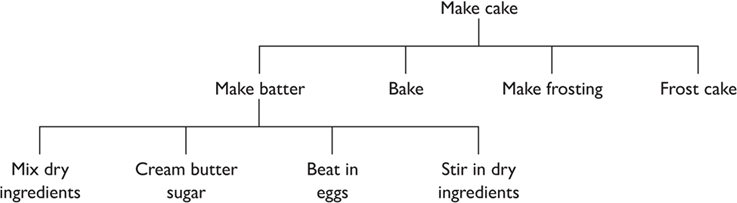
\includegraphics[width=0.92\textwidth,height=0.32\textheight,keepaspectratio]{images/fig1_2_make_cake_decomposition.png}\\[1mm]
    \tiny\textit{Hình 1.2: Sơ đồ cấu trúc phân rã tác vụ làm bánh (Trích giáo trình Chapter 1, Trang 66)}
  \end{center}

  \begin{columns}
    \column{0.5\textwidth}
    \begin{tcolorbox}[colback=white,colframe=UniBlue,title=\textbf{Đặc điểm của Sơ đồ Cấu trúc (Structure Diagram)}]
      \small
      \begin{itemize}
        \item \textbf{Cấp cao nhất (Top level):} Nhiệm vụ tổng thể (\textit{Make cake}).
        \item \textbf{Cấp 1:} Các giai đoạn chính (\textit{Make batter}, \textit{Bake}, \textit{Make frosting}, \textit{Frost cake}).
        \item \textbf{Cấp 2:} Thao tác cụ thể (\textit{Mix dry ingredients}, \textit{Cream butter and sugar}...).
      \end{itemize}
    \end{tcolorbox}

    \column{0.5\textwidth}
    \begin{exampleblock}{\textbf{Ý nghĩa sư phạm trong lập trình}}
      \begin{itemize}\small
        \item Giúp người lập trình có cái nhìn tổng quan trước khi viết từng dòng code.
        \item Trong Java, mỗi hộp trong sơ đồ cấu trúc sẽ tương ứng với một \textbf{phương thức tĩnh (static method)}.
      \end{itemize}
    \end{exampleblock}
  \end{columns}
\end{frame}

% ------------------------------------------------------------------------------
\begin{frame}[fragile]{Phương thức tĩnh (Static Methods): Cú pháp Khai báo \& Lời gọi}
  \begin{columns}[t]
    \column{0.5\textwidth}
    \begin{block}{\textbf{Cú pháp Khai báo (Declaring a Method)}}
      Định nghĩa tên và hành vi của phương thức:
      \begin{lstlisting}
public static void <tenPhuongThuc>() {
    <cac cau lenh thuc thi>;
}
      \end{lstlisting}
      \textit{Ví dụ:}
      \begin{lstlisting}
public static void drawBox() {
    System.out.println("+------+");
    System.out.println("|      |");
    System.out.println("|      |");
    System.out.println("+------+");
}
      \end{lstlisting}
    \end{block}

    \column{0.5\textwidth}
    \begin{block}{\textbf{Cú pháp Lời gọi (Calling a Method)}}
      Ra lệnh cho máy tính thực thi phương thức:
      \begin{lstlisting}
<tenPhuongThuc>();
      \end{lstlisting}
      \textit{Ví dụ trong \texttt{main}:}
      \begin{lstlisting}
public static void main(String[] args) {
    drawBox(); // Goi lan 1
    System.out.println();
    drawBox(); // Goi lan 2 (Tai su dung!)
}
      \end{lstlisting}
    \end{block}
  \end{columns}

  \vspace{1mm}
  \begin{alertblock}{\textbf{Lưu ý:}}
    Không được khai báo một phương thức nằm bên trong thân của một phương thức khác! Mọi phương thức phải nằm trực tiếp bên trong lớp (\texttt{class}).
  \end{alertblock}
\end{frame}

% ------------------------------------------------------------------------------
\begin{frame}{Luồng điều khiển khi gọi phương thức (Flow of Control)}
  \begin{columns}
    \column{0.55\textwidth}
    \begin{center}
      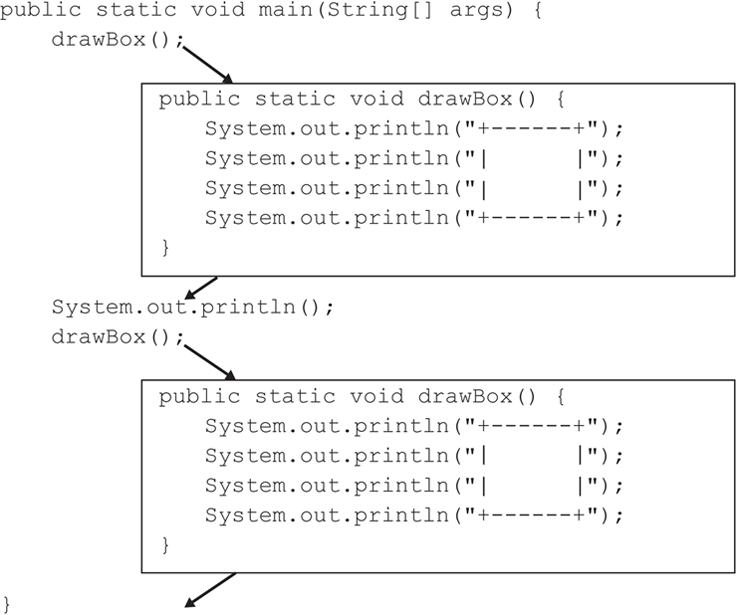
\includegraphics[width=0.95\textwidth,height=0.75\textheight,keepaspectratio]{images/fig_flow_of_control_drawboxes.png}\\[1mm]
      \tiny\textit{Sơ đồ luồng điều khiển chương trình DrawBoxes (Trích giáo trình Chapter 1, Trang 76)}
    \end{center}

    \column{0.45\textwidth}
    \begin{block}{\textbf{Quy tắc chuyển giao điều khiển:}}
      \begin{enumerate}\footnotesize
        \item Chương trình \textbf{luôn bắt đầu} tại dòng đầu tiên của hàm \texttt{main}.
        \item Khi gặp lời gọi hàm (\texttt{drawBox();}):
          \begin{itemize}\scriptsize
            \item Máy tính \textbf{tạm dừng} thực thi tại \texttt{main}.
            \item Nhảy tới thân phương thức \texttt{drawBox} và thực thi tuần tự các lệnh trong đó.
          \end{itemize}
        \item Khi phương thức chạy xong dấu ngoặc đóng \texttt{\}}:
          \begin{itemize}\scriptsize
            \item Quyền điều khiển quay trở lại (\textbf{return}) đúng vị trí vừa rời đi ở \texttt{main}.
            \item Tiếp tục thực thi câu lệnh kế tiếp!
          \end{itemize}
      \end{enumerate}
    \end{block}
  \end{columns}
\end{frame}

% ------------------------------------------------------------------------------
\begin{frame}{Luồng điều khiển đa cấp \& Khái niệm Ngăn xếp gọi hàm (Call Stack)}
  \begin{columns}
    \column{0.5\textwidth}
    \begin{center}
      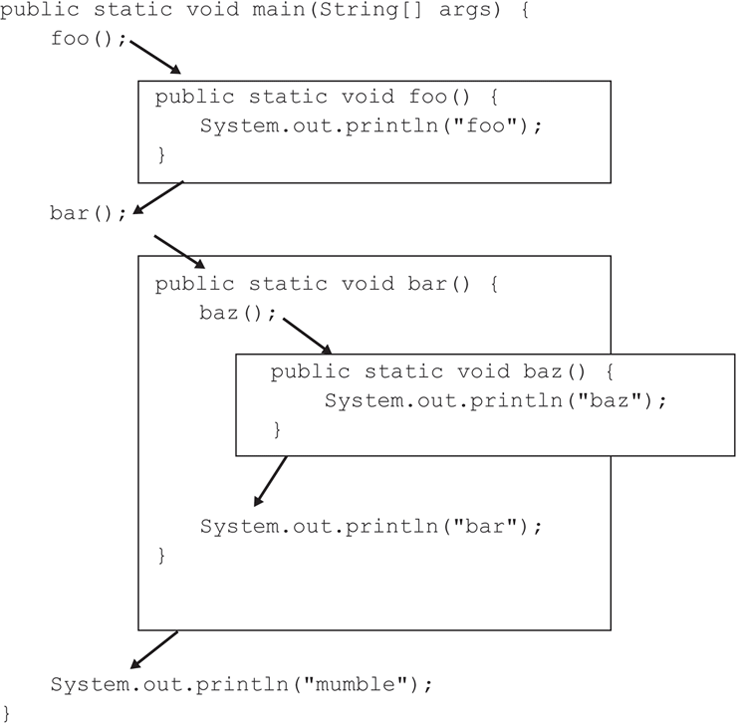
\includegraphics[width=0.98\textwidth,height=0.68\textheight,keepaspectratio]{images/fig_control_flow_step2.png}\\[1mm]
      \tiny\textit{Sự mở rộng luồng điều khiển lồng nhau foo $\to$ bar $\to$ baz (Trang 82)}
    \end{center}

    \column{0.5\textwidth}
    \begin{block}{\textbf{Cơ chế hoạt động của Call Stack}}
      \begin{itemize}\footnotesize
        \item Một phương thức có thể gọi một phương thức khác (\texttt{bar()} gọi \texttt{baz()}).
        \item Máy tính ghi nhớ thứ tự quay về bằng cấu trúc \textbf{Ngăn xếp (Call Stack - LIFO: Vào sau ra trước)}.
        \item Khi \texttt{baz()} chạy xong $\to$ quay về \texttt{bar()} $\to$ \texttt{bar()} chạy xong $\to$ quay về \texttt{main}.
      \end{itemize}
    \end{block}

    \begin{alertblock}{\textbf{Lợi ích kép của Phân rã thủ tục:}}
      \begin{enumerate}\footnotesize
        \item \textbf{Structure (Cấu trúc):} Biến chương trình dài phức tạp thành các module ngắn gọn, dễ hiểu.
        \item \textbf{Eliminate Redundancy (Xóa bỏ trùng lặp):} Viết 1 lần, gọi thực thi vô số lần!
      \end{enumerate}
    \end{alertblock}
  \end{columns}
\end{frame}

% ------------------------------------------------------------------------------
\begin{frame}[fragile]{1.5 Case Study: Bài toán vẽ hình ASCII nghệ thuật (DrawFigures)}
  \begin{columns}
    \column{0.45\textwidth}
    \begin{tcolorbox}[colback=white,colframe=UniNavy,title=\textbf{Yêu cầu bài toán (Output mong đợi)}]
      Viết chương trình in ra 3 hình đồ họa ký tự ASCII:
      \begin{enumerate}
        \item \textbf{Hình Kim cương (Diamond)}
        \item \textbf{Hình Chữ X (X)}
        \item \textbf{Hình Tên lửa vũ trụ (Rocket)}
      \end{enumerate}
      Các hình cách nhau một dòng trống.
    \end{tcolorbox}

    \column{0.55\textwidth}
    \textbf{Hình ảnh ASCII thực tế xuất ra Console:}
    \begin{lstlisting}[style=terminalStyle]
   /\          \    /          /\ 
  /  \          \  /          /  \ 
 /    \          \/          /    \ 
 \    /          /\         +------+
  \  /          /  \        |      |
   \/          /    \       |      |
                            +------+
                            |      |
                            |      |
                            +------+
                               /\ 
                              /  \ 
                             /    \ 
    \end{lstlisting}
  \end{columns}
\end{frame}

% ------------------------------------------------------------------------------
\begin{frame}[fragile]{Phiên bản 1 (DrawFigures1): Tiếp cận Ngây thơ (Naïve Approach)}
  \begin{columns}
    \column{0.55\textwidth}
    \begin{lstlisting}[caption={DrawFigures1.java (Trích đoạn)}]
public class DrawFigures1 {
    public static void main(String[] args) {
        // Ve kim cuong (Diamond)
        System.out.println("   /\\");
        System.out.println("  /  \\");
        System.out.println(" /    \\");
        System.out.println(" \\    /");
        System.out.println("  \\  /");
        System.out.println("   \\/");
        System.out.println();
        // Ve chu X
        System.out.println(" \\    /");
        System.out.println("  \\  /");
        System.out.println("   \\/");
        System.out.println("   /\\");
        // ... tiep tuc hang chuc dong lenh!
    }
}
    \end{lstlisting}

    \column{0.45\textwidth}
    \begin{alertblock}{\textbf{Đánh giá chất lượng thiết kế:}}
      \begin{itemize}\small
        \item \textbf{Số dòng lệnh:} Hơn 30 dòng lệnh \texttt{println} dồn hết vào hàm \texttt{main}.
        \item \textbf{Trùng lặp trầm trọng:} Cụm nón trên (\textit{cone}) lặp lại 3 lần. Cụm nón dưới (\textit{v}) lặp lại 2 lần. Cụm hình hộp lặp lại 2 lần.
        \item \textbf{Hậu quả bảo trì:} Nếu muốn mở rộng hình rộng hơn 1 dấu cách, ta phải đi sửa thủ công ở hàng chục vị trí khác nhau!
      \end{itemize}
    \end{alertblock}
    \vspace{2mm}
    \centering
    $\to$ \textbf{Cần áp dụng Phân rã thủ tục cấp 1!}
  \end{columns}
\end{frame}

% ------------------------------------------------------------------------------
\begin{frame}{Phiên bản 2 (DrawFigures2): Phân rã Cấp 1 theo Khối hình}
  \begin{center}
    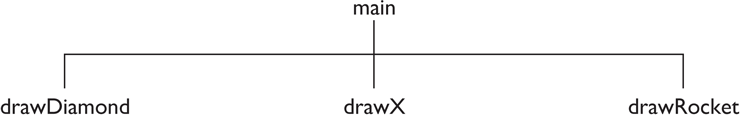
\includegraphics[width=0.88\textwidth,height=0.18\textheight,keepaspectratio]{images/fig1_3_drawfigures2_decomposition.png}\\[1mm]
    \tiny\textit{Hình 1.3: Sơ đồ cấu trúc phân rã cấp 1 của DrawFigures2 (Trích giáo trình Chapter 1, Trang 92)}
  \end{center}

  \begin{columns}[t]
    \column{0.5\textwidth}
    \begin{exampleblock}{\textbf{Cải tiến ở Phiên bản 2:}}
      \begin{itemize}\footnotesize
        \item Tách \texttt{main} thành 3 phương thức con:
          \begin{itemize}\scriptsize
            \item \texttt{drawDiamond()}
            \item \texttt{drawX()}
            \item \texttt{drawRocket()}
          \end{itemize}
        \item Hàm \texttt{main} bây giờ cực kỳ ngắn gọn và sáng sủa:
          \begin{center}\scriptsize
            \texttt{drawDiamond(); drawX(); drawRocket();}
          \end{center}
      \end{itemize}
    \end{exampleblock}

    \column{0.5\textwidth}
    \begin{alertblock}{\textbf{Hạn chế vẫn còn tồn tại:}}
      \begin{itemize}\footnotesize
        \item Bên trong thân của \texttt{drawDiamond}, \texttt{drawX}, và \texttt{drawRocket}, các câu lệnh in nón xuôi (\texttt{/\textbackslash}) và nón ngược (\texttt{\textbackslash/}) \textbf{vẫn bị lặp lại}!
        \item \textbf{Giải pháp triệt để:} Tiếp tục phân rã xuống cấp thứ 2 thành các hình khối cơ sở (\textit{primitives})!
      \end{itemize}
    \end{alertblock}
  \end{columns}
\end{frame}

% ------------------------------------------------------------------------------
\begin{frame}{Phiên bản 3 (DrawFigures3): Phân rã Hoàn chỉnh 2 Cấp (Triệt tiêu trùng lặp)}
  \begin{center}
    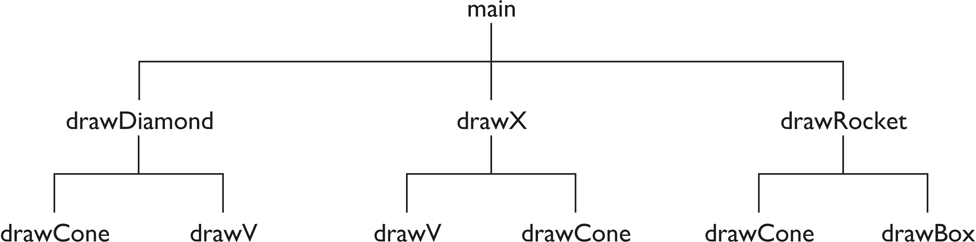
\includegraphics[width=0.92\textwidth,height=0.28\textheight,keepaspectratio]{images/fig1_4_drawfigures3_decomposition.png}\\[1mm]
    \tiny\textit{Hình 1.4: Sơ đồ cấu trúc phân rã hoàn chỉnh 2 cấp của DrawFigures3 (Trích giáo trình Chapter 1, Trang 96)}
  \end{center}

  \begin{tcolorbox}[colback=white,colframe=UniGreen,title=\textbf{Cấu trúc 3 tầng chuẩn kiến trúc phần mềm:}]
    \footnotesize
    \begin{itemize}
      \item \textbf{Tầng 1 (Điều phối):} Phương thức \texttt{main()} nắm giữ bức tranh toàn cảnh cấp cao nhất.
      \item \textbf{Tầng 2 (Khối hình hoàn chỉnh):} \texttt{drawDiamond()}, \texttt{drawX()}, \texttt{drawRocket()}.
      \item \textbf{Tầng 3 (Các khối nguyên thủy tái sử dụng):} \texttt{drawCone()} (Nón trên), \texttt{drawV()} (Nón dưới), \texttt{drawBox()} (Thân hộp).
    \end{itemize}
  \end{tcolorbox}
\end{frame}

% ------------------------------------------------------------------------------
\begin{frame}[fragile]{Mã nguồn hoàn chỉnh đạt chuẩn: \texttt{DrawFigures3.java}}
  \begin{columns}[t]
    \column{0.48\textwidth}
    \begin{lstlisting}[caption={Tầng 1 \& Tầng 2}]
public class DrawFigures3 {
    public static void main(String[] args) {
        drawDiamond();
        System.out.println();
        drawX();
        System.out.println();
        drawRocket();
    }
    public static void drawDiamond() {
        drawCone();
        drawV();
    }
    public static void drawX() {
        drawV();
        drawCone();
    }
    public static void drawRocket() {
        drawCone();
        drawBox();
        drawBox();
        drawCone();
    }
    \end{lstlisting}

    \column{0.48\textwidth}
    \begin{lstlisting}[caption={Tầng 3 (Primitives Reusable)}]
    public static void drawCone() {
        System.out.println("   /\\");
        System.out.println("  /  \\");
        System.out.println(" /    \\");
    }
    public static void drawV() {
        System.out.println(" \\    /");
        System.out.println("  \\  /");
        System.out.println("   \\/");
    }
    public static void drawBox() {
        System.out.println("+------+");
        System.out.println("|      |");
        System.out.println("|      |");
        System.out.println("+------+");
    }
}
    \end{lstlisting}
  \end{columns}
\end{frame}

% ------------------------------------------------------------------------------
\begin{frame}{So sánh \& Đánh giá 3 thế hệ thiết kế}
  \centering
  \small
  \begin{tabularx}{0.96\textwidth}{l X X X}
    \toprule
    \textbf{Tiêu chí đánh giá} & \textbf{DrawFigures1 (Naïve)} & \textbf{DrawFigures2 (Cấp 1)} & \textbf{DrawFigures3 (Cấp 2)} \\
    \midrule
    \textbf{Cấu trúc mã nguồn} & Rối rắm, nguyên khối 1 hàm duy nhất. & Tách biệt từng hình lớn, dễ theo dõi hơn. & Phân tầng rõ rệt: Điều phối - Lắp ráp - Nguyên tử. \\
    \addlinespace
    \textbf{Mức độ trùng lặp} & Rất cao (\textit{Heavy redundancy}). & Vẫn lặp code vẽ nón và vẽ hộp. & \textbf{Triệt tiêu 100\%} trùng lặp code in hình. \\
    \addlinespace
    \textbf{Khả năng tái sử dụng} & 0\% (phải copy-paste dòng lệnh). & Chỉ tái sử dụng được cả hình kim cương hay chữ X. & \textbf{Tái sử dụng tối đa} mọi khối nguyên thủy. \\
    \addlinespace
    \textbf{Khả năng bảo trì} & Sửa đổi 1 chi tiết phải sửa hàng chục chỗ. & Vẫn phải sửa nhiều nơi. & \textbf{Chỉ cần sửa 1 chỗ duy nhất} tại khối nguyên thủy! \\
    \bottomrule
  \end{tabularx}
\end{frame}

% ------------------------------------------------------------------------------
\begin{frame}[fragile]{[CHECKPOINT 3] Dự đoán luồng thực thi hàm lồng nhau}
  \begin{columns}
    \column{0.55\textwidth}
    \begin{lstlisting}
public class TraceTest {
    public static void main(String[] args) {
        first();
        second();
    }
    public static void first() {
        System.out.println("1");
    }
    public static void second() {
        System.out.println("2");
        first();
        System.out.println("3");
    }
}
    \end{lstlisting}

    \column{0.45\textwidth}
    \begin{exampleblock}{\textbf{Thứ tự in trên màn hình là gì?}}
      \begin{enumerate}[A.]
        \item 1, 2, 3
        \item 1, 2, 1, 3
        \item 1, 2, 3, 1
        \item 2, 1, 3
      \end{enumerate}
    \end{exampleblock}

    \begin{tcolorbox}[colback=white,colframe=UniBlue,title=\textbf{Giải thích:}]
      \footnotesize
      1. \texttt{main} gọi \texttt{first()} $\to$ in \textbf{1}.\\
      2. \texttt{main} gọi \texttt{second()}:\\
      \quad - In \textbf{2}.\\
      \quad - Gọi \texttt{first()} $\to$ in \textbf{1}.\\
      \quad - In \textbf{3}.\\
      $\to$ \textbf{Đáp án chính xác: B (1, 2, 1, 3)}
    \end{tcolorbox}
  \end{columns}
\end{frame}

% ------------------------------------------------------------------------------
\begin{frame}[fragile]{[HANDS-ON LAB 3] Mini-Project: Thiết kế chương trình Rocket/FightSong}
  \begin{tcolorbox}[colback=white,colframe=UniGreen,title=\textbf{Mini Project Tiết 3 (Thời gian: 20 phút -- Đánh giá sản phẩm tại lớp)}]
    \small
    \textbf{Đề bài (Chọn 1 trong 2):}
    \begin{itemize}\footnotesize
      \item \textbf{Lựa chọn A (Đồ họa ASCII):} Viết \texttt{SpaceRocket.java} vẽ một trạm không gian gồm 2 tên lửa đứng cạnh nhau, mỗi tên lửa gồm mũi nhọn, thân chứa biểu tượng \texttt{IT26M}, khoang động cơ, và ngọn lửa đáy. Yêu cầu \textbf{triệt tiêu 100\% trùng lặp}.
      \item \textbf{Lựa chọn B (Bài hát cổ động - Exercise 12, p.125):} Viết chương trình \texttt{FightSong.java} in lời bài hát có các điệp khúc lặp lại bằng cách phân rã thành ít nhất 2 phương thức tĩnh phụ ngoài \texttt{main}.
    \end{itemize}
  \end{tcolorbox}

  \begin{columns}
    \column{0.5\textwidth}
    \textbf{Tiêu chí chấm điểm Lab:}
    \begin{enumerate}\scriptsize
      \item Biên dịch và chạy hoàn hảo (\texttt{0 errors, 0 warnings}).
      \item Cấu trúc phân rã rõ ràng (Tối thiểu 2 cấp phân rã).
      \item Tuân thủ chuẩn đặt tên CamelCase và chú thích code.
    \end{enumerate}

    \column{0.5\textwidth}
    \begin{exampleblock}{\textbf{Cấu trúc mẫu SpaceRocket:}}
      \begin{itemize}\scriptsize
        \item \texttt{drawNoseCone()}
        \item \texttt{drawBodySegment()}
        \item \texttt{drawThruster()}
        \item \texttt{drawFlame()}
      \end{itemize}
    \end{exampleblock}
  \end{columns}
\end{frame}

% ==============================================================================
% PHẦN TỔNG KẾT
% ==============================================================================
\section{Tổng kết \& Hướng dẫn Tự học}

\begin{frame}{Tổng kết toàn bộ kiến thức Chương 1 (Checklist Chuẩn đầu ra)}
  \centering
  \small
  \begin{tabularx}{0.98\textwidth}{l X c}
    \toprule
    \textbf{Mục tiêu CLO} & \textbf{Kiến thức cốt lõi đã làm chủ trong 3 tiết} & \textbf{Trạng thái} \\
    \midrule
    \textbf{CLO 1.1} & Hiểu phần cứng, nhị phân, vai trò của Bytecode và máy ảo JVM (WORA). & \checkmark \\
    \addlinespace
    \textbf{CLO 1.2} & Viết đúng cấu trúc class, hàm \texttt{main}, phân biệt \texttt{print}/\texttt{println}, dùng thành thạo ký tự thoát (\texttt{\textbackslash n, \textbackslash t, \textbackslash", \textbackslash\textbackslash}). & \checkmark \\
    \addlinespace
    \textbf{CLO 1.3} & Nhận diện và phân biệt 3 loại lỗi: Cú pháp (Syntax), Thực thi (Runtime), Ngữ nghĩa (Logic); đọc hiểu thông báo lỗi compiler. & \checkmark \\
    \addlinespace
    \textbf{CLO 1.4} & Nắm vững tư duy phân rã Top-down; khai báo và gọi phương thức tĩnh; hiểu luồng điều khiển và ngăn xếp gọi hàm. & \checkmark \\
    \addlinespace
    \textbf{CLO 1.5} & Viết mã nguồn có cấu trúc module chuẩn, áp dụng nguyên lý DRY, biên dịch và chạy độc lập trên CLI và IDE. & \checkmark \\
    \bottomrule
  \end{tabularx}
\end{frame}

% ------------------------------------------------------------------------------
\begin{frame}{Bảng tra cứu nhanh cú pháp cốt lõi (Java Quick Cheatsheet)}
  \begin{columns}[t]
    \column{0.5\textwidth}
    \begin{tcolorbox}[colback=white,colframe=UniNavy,title=\textbf{Cấu trúc chương trình \& Xuất màn hình}]
      \footnotesize
      \textbf{Khung chương trình:}\\
      \texttt{public class TênLớp \{}\\
      \quad\texttt{public static void main(String[] args) \{}\\
      \qquad\texttt{System.out.println("Nội dung");}\\
      \quad\texttt{\}}\\
      \texttt{\}}\\[2mm]
      \textbf{Ký tự thoát:}\\
      \texttt{\textbackslash n} (Xuống dòng) \quad \texttt{\textbackslash t} (Tab)\\
      \texttt{\textbackslash"} (Dấu ngoặc kép) \quad \texttt{\textbackslash\textbackslash} (Gạch chéo ngược)
    \end{tcolorbox}

    \column{0.5\textwidth}
    \begin{tcolorbox}[colback=white,colframe=UniBlue,title=\textbf{Phương thức tĩnh \& Phân rã}]
      \footnotesize
      \textbf{Khai báo hàm:}\\
      \texttt{public static void tênHàm() \{}\\
      \quad\texttt{... các câu lệnh ...}\\
      \texttt{\}}\\[2mm]
      \textbf{Lời gọi hàm:}\\
      \texttt{tênHàm();}\\[2mm]
      \textbf{Quy tắc vàng:}\\
      - Hàm không được lồng trong hàm khác.\\
      - Đặt tên theo chuẩn \texttt{lowerCamelCase}.\\
      - Triệt tiêu trùng lặp code (DRY).
    \end{tcolorbox}
  \end{columns}
\end{frame}

% ------------------------------------------------------------------------------
\begin{frame}{Nhiệm vụ tự học \& Bài tập về nhà cho lớp IT26M}
  \begin{columns}[t]
    \column{0.5\textwidth}
    \begin{block}{\textbf{1. Bài tập bắt buộc (Nộp trên hệ thống LMS)}}
      \begin{itemize}\small
        \item Đọc lại toàn bộ Chương 1 giáo trình (Trang 1 -- 102).
        \item Làm các câu hỏi \textbf{Self-Check}:
          \begin{itemize}\footnotesize
            \item Câu 6, 8, 10, 13 (Cú pháp \& Escape Seq).
            \item Câu 18, 19 (Tìm lỗi chương trình).
            \item Câu 24, 26, 27 (Luồng điều khiển).
          \end{itemize}
        \item Lập trình \textbf{Exercise 7 (Mantra)} và \textbf{Exercise 11 (TwoRockets)} trang 122--125.
      \end{itemize}
    \end{block}

    \column{0.5\textwidth}
    \begin{block}{\textbf{2. Bài tập thử thách (Cộng điểm chuyên cần)}}
      \begin{itemize}\small
        \item \textbf{Programming Project 1 (MISSISSIPPI):} In chữ MISSISSIPPI dạng khối lớn (Block letters) với phân rã tối ưu (p.130).
        \item \textbf{Programming Project 3:} Bài hát dân gian tích lũy điệp khúc có cấu trúc phân tầng (p.131).
      \end{itemize}
    \end{block}
    \vspace{1mm}
    \begin{alertblock}{\textbf{Chuẩn bị cho Buổi học kế tiếp:}}
      \small Đọc trước \textbf{Chương 2: Primitive Data and Definite Loops} (Biến, Kiểu số nguyên/thực, Biểu thức toán học, và Vòng lặp \texttt{for}).
    \end{alertblock}
  \end{columns}
\end{frame}

% ------------------------------------------------------------------------------
\begin{frame}[plain]
  \begin{center}
    \vspace{1.5cm}
    {\Huge \textcolor{UniNavy}{\textbf{CẢM ƠN CÁC BẠN SINH VIÊN LỚP IT26M!}}}\\[6mm]
    {\Large \textbf{HỎI ĐÁP \& THẢO LUẬN (Q\&A)}}\\[4mm]
    \rule{0.4\textwidth}{1pt}\\[4mm]
    \textit{Chúc các bạn có những giờ học lập trình Java say mê và hiệu quả!}\\[8mm]
    \small Khoa Công nghệ Thông tin -- Đại học UDA
  \end{center}
\end{frame}

\end{document}
